\documentclass[12pt]{article}

\usepackage[margin=1in]{geometry}
\usepackage{amsmath,amssymb,booktabs,array,graphicx,float,fancyhdr,setspace,hyperref,xcolor,longtable,enumitem}
\usepackage{caption,etoolbox,calc,fvextra}
\usepackage[T1]{fontenc}
\usepackage[utf8]{inputenc}
\usepackage{lmodern}

\definecolor{linkblue}{RGB}{0,72,135}
\hypersetup{
    colorlinks=true,
    linkcolor=linkblue,
    urlcolor=linkblue,
    citecolor=linkblue,
    pdftitle={Airport Code Lookup Service with a Binary Search Tree},
    pdfauthor={Yasmein Asfour and Ayham Makhamra}
}

\setstretch{1.15}
\setlength{\parindent}{0pt}
\setlength{\parskip}{6pt}
\setlength{\headheight}{15pt}
\pagestyle{fancy}
\fancyhf{}
\fancyhead[L]{EECE 2560}
\fancyhead[R]{Airport BST Mini Project}
\fancyfoot[C]{\thepage}
\setlist[itemize]{itemsep=2pt,topsep=3pt}
\captionsetup{font=small,labelfont=bf}
\setlength{\emergencystretch}{3em}

\begin{document}

\begin{titlepage}
    \centering
    \vspace*{0.8in}
    {\Large Northeastern University\par}
    \vspace{0.15in}
    {\large College of Engineering\par}
    \vspace{0.5in}
    {\large EECE 2560: Fundamentals of Engineering Algorithms\par}
    \vfill
    {\Huge\bfseries Airport Code Lookup Service\par}
    \vspace{0.18in}
    {\LARGE Using a Binary Search Tree\par}
    \vspace{0.35in}
    {\Large Mini Project Report\par}
    \vfill
    {\large Yasmein Asfour\\[0.08in]Ayham Makhamra\par}
    \vspace{0.15in}
    {\large Fall 2026\par}
    \vspace*{0.8in}
\end{titlepage}

\tableofcontents
\newpage

\section{Abstract}

In this project, we built an airport lookup program in C++17 using a binary search tree (BST). Each airport is stored by its three-letter IATA code. The program can load the OpenFlights data, find airports, add or remove records, print the airports in order, search within a range, and check that the tree is still valid. It can also save and reload the tree and rebuild it in a balanced shape. We tested all of the required operations, including the three deletion cases. We also compared different tree shapes to see how insertion order affects search speed.

\section{Introduction}

Airports usually have a three-letter IATA code, so the code works well as a key. In a BST, smaller codes go to the left and larger codes go to the right. This lets the program follow one path through the tree instead of checking every airport. How fast this works depends on the shape of the tree.

The main goal was to take the BST algorithms from class and use them in a working command-line program. The program also prints search paths, deletion cases, tree height, and average depth. These values helped us see what was happening inside the tree and made the program easier to test.

\section{Objectives}

For this project, we wanted the program to:

\begin{itemize}
    \item Load valid airport records from the supplied OpenFlights data file.
    \item Store airports in a BST ordered by IATA code.
    \item Support searching, insertion, deletion, sorted listing, and range queries.
    \item Handle leaf, one-child, and two-child deletion cases correctly.
    \item Validate the BST using lower and upper key limits.
    \item Save a tree in preorder and rebuild the same shape later.
    \item Rebalance the tree using the middle element of a sorted list.
    \item Compare the shape and search performance of different insertion orders.
\end{itemize}

\section{Program Design}

\subsection{Main data structures}

The \texttt{Airport} class stores the information for one airport: IATA code, name, city, country, ICAO code, latitude, and longitude. The \texttt{AirportBST} class manages the tree. Each node stores one \texttt{Airport} and has pointers to a left child and a right child.

We use the IATA code as the key. When searching or inserting, the program compares the codes alphabetically. It goes left for a smaller code and right for a larger code. If the code is already in the tree, it is not added again.

\begin{table}[H]
\centering
\caption{Main project files and their responsibilities.}
\begin{tabular}{@{}p{0.30\textwidth}p{0.62\textwidth}@{}}
\toprule
\textbf{File} & \textbf{Purpose} \\
\midrule
\texttt{src/Airport.h/.cpp} & Defines an airport record and its output format. \\
\texttt{src/AirportBST.h/.cpp} & Implements the BST operations and tree measurements. \\
\texttt{src/main.cpp} & Loads data and provides the command-line interface. \\
\texttt{tests/run\_tests.sh} & Builds the program and checks the required behavior. \\
\texttt{docs/pseudocode.md} & Describes the main algorithms before implementation. \\
\bottomrule
\end{tabular}
\end{table}

\subsection{Loading the data}

The loader reads the airport file one record at a time and handles commas inside quoted text. If the IATA field is \texttt{\textbackslash N}, the record is skipped because there is no code to use as a key. The valid airports are inserted in the same order they appear in the file. There are 7,698 lines total. Out of those, 6,072 have valid IATA codes and 1,626 are skipped. The data did not contain any duplicate valid IATA codes.

\subsection{Searching and insertion}

Searching starts at the root. After each comparison, the program goes either left or right. It prints every code it visits so we can see the full search path. Insertion works in almost the same way, but it stops at an empty spot and puts the new node there.

Search and insertion take $O(h)$ time, where $h$ is the height of the tree. In a balanced tree, the height is close to $\log_2 n$. In the worst case, the tree can turn into a long chain with height $n-1$.

\subsection{Deletion}

To delete an airport, the program first searches for its code. Then it handles one of these three cases:

\begin{itemize}
    \item \textbf{D1: leaf.} The node has no children and can be removed directly.
    \item \textbf{D2: one child.} The node is replaced by its only child.
    \item \textbf{D3: two children.} The smallest node in the right subtree is found. Its airport record replaces the deleted record, and the successor node is then removed.
\end{itemize}

These steps keep the tree in the correct order. The program prints D1, D2, or D3 so we can tell which case happened.

\subsection{Traversal, validation, and rebalancing}

An inorder traversal visits the left side, the current node, and then the right side. This prints all airport codes in alphabetical order. The range command uses the same idea, but it skips parts of the tree that cannot have a code in the requested range.

The validation function keeps a lower and upper limit for every recursive call. A node has to be between those limits. To rebalance the tree, the program first puts the records in sorted order. It picks the middle record as the root and repeats the same step on the left and right halves.

\begin{table}[H]
\centering
\caption{Time complexity of the main operations.}
\begin{tabular}{@{}p{0.31\textwidth}p{0.18\textwidth}>{\raggedright\arraybackslash}p{0.39\textwidth}@{}}
\toprule
\textbf{Operation} & \textbf{Time} & \textbf{Reason} \\
\midrule
Search, insert, or delete & $O(h)$ & At most one path from the root is followed. \\
Inorder listing & $O(n)$ & Every node is visited once. \\
Range query & $O(h+k)$ & Unneeded branches are pruned; $k$ results are printed. \\
Validation & $O(n)$ & Each node is checked once. \\
Balanced rebuild & $O(n)$ & Each sorted record becomes one node. \\
\bottomrule
\end{tabular}
\end{table}

\section{User Interface}

The program uses a simple text command loop. Some of the main commands are \texttt{load}, \texttt{find}, \texttt{add}, \texttt{remove}, \texttt{list}, \texttt{range}, \texttt{save}, \texttt{validate}, \texttt{rebalance}, and \texttt{experiment}. We used commands because they make each BST operation easy to run and show during the demo.

The project can be built and started with:

\begin{Verbatim}[fontsize=\small,frame=single]
g++ -std=c++17 -O2 src/*.cpp -o airports
./airports
\end{Verbatim}

After the program starts, the data is loaded with:

\begin{Verbatim}[fontsize=\small,frame=single]
load data/airports.dat
\end{Verbatim}

\section{Testing}

\subsection{Testing method}

The test script builds the program and checks the main features. It tests loading, searching, adding, all deletion cases, range output, preorder save/reload, validation, and rebalancing. For each deletion case, the original tree is loaded again. This keeps one deletion from changing the setup for another test.

We used the following airport codes to check specific parts of the original tree:

\begin{table}[H]
\centering
\caption{Representative test cases from the original file-order tree.}
\begin{tabular}{@{}p{0.38\textwidth}p{0.17\textwidth}p{0.34\textwidth}@{}}
\toprule
\textbf{Test} & \textbf{Code} & \textbf{Expected result} \\
\midrule
Root & \texttt{GKA} & Found at the root \\
Leaf deletion & \texttt{AAC} & D1 \\
Only left child & \texttt{GJT} & D2, child \texttt{GJR} \\
Only right child & \texttt{AAA} & D2, child \texttt{AAC} \\
Two children & \texttt{AEY} & D3, successor \texttt{AFA} \\
Deep search & \texttt{YZR} & Depth 177 \\
Missing code & \texttt{XYZ} & Not found \\
Minimum and maximum & \texttt{AAA}, \texttt{ZZV} & Correct endpoints \\
\bottomrule
\end{tabular}
\end{table}

\subsection{Automated test result}

Figure~\ref{fig:tests} shows the final test run. The script finished with the message \texttt{All Airport BST tests passed.}

\begin{figure}[H]
    \centering
    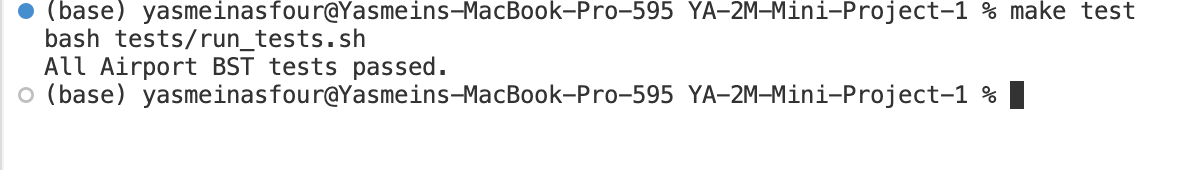
\includegraphics[width=0.96\textwidth]{assets/tests-passed.png}
    \caption{Terminal output from \texttt{make test}.}
    \label{fig:tests}
\end{figure}

\section{Results}

\subsection{Original tree}

When we loaded the airports in file order, the tree had 6,072 nodes, a height of 177, and an average depth of 18.323. The root was \texttt{GKA}. Finding \texttt{BOS} took 12 comparisons and followed this path:

\begin{Verbatim}[fontsize=\small,frame=single,breaklines=true]
GKA -> AEY -> EGS -> BUJ -> BJA -> BSK -> BOY -> BNI
    -> BOH -> BOO -> BOU -> BOS
\end{Verbatim}

The range from \texttt{BOS} through \texttt{BWI} returned 113 airports and visited 127 nodes. It did not need to check all 6,072 nodes because it skipped branches outside the range.

After saving the original tree in preorder and loading it again, it had the same height and the same first three levels:

\begin{Verbatim}[fontsize=\small,frame=single]
Level 0: GKA
Level 1: AEY MAG
Level 2: AAE EGS HGU POM
\end{Verbatim}

\subsection{Tree-shape experiment}

We built the tree three times using different insertion orders. Table~\ref{tab:experiment} shows the results from our final run. The exact times can change a little depending on the computer.

\begin{table}[H]
\centering
\caption{Effect of insertion order on tree shape and search time.}
\label{tab:experiment}
\begin{tabular}{@{}lrrr@{}}
\toprule
\textbf{Build order} & \textbf{Height} & \textbf{Average depth} & \textbf{10,000 searches} \\
\midrule
File order & 177 & 18.323 & 4.677 ms \\
Sorted order & 6,071 & 3,035.500 & 316.810 ms \\
Balanced middle rule & 12 & 10.653 & 3.061 ms \\
\bottomrule
\end{tabular}
\end{table}

When the records were already sorted, every new code went to the right. This made the tree one long chain, so it had the worst height and search time. The balanced tree had a height close to $\log_2(6072)$ and was the fastest. The file-order tree worked much better than the sorted tree, but it was still taller than the balanced tree.

\section{Demonstration Videos}

We split the project demonstration into two videos:

\begin{itemize}
    \item \textbf{Demo Part 1:} \url{https://youtu.be/7mMD7evsa1c}
    \item \textbf{Demo Part 2:} \url{https://youtu.be/LFwiUs4Al4c?si=Xs-r1mi-l-U9g9WG}
\end{itemize}

The links are clickable in the PDF.

\section{Discussion}

The biggest thing we learned was that the shape of the tree matters a lot. BST search is $O(h)$, not always $O(\log n)$, because the tree is not automatically balanced. The sorted-order test showed this clearly. The tree was still a valid BST, but it worked like a linked list and searches took much longer.

Deletion was the part that needed the most attention because the pointers have to be changed without losing part of the tree. Printing D1, D2, or D3 made it easier to check each case. Running validation after changes was also helpful because it checked the ordering of the whole tree.

One limitation is that the preorder save file only stores IATA codes. The original airport data has to be loaded first so the program can match those codes to the full records. This was enough for the assignment because the goal was to recreate the shape of the tree.

\section{Conclusion}

In the end, our program loaded the airport data and completed all of the required BST operations. The automated tests passed for searching, adding, every deletion case, traversal, ranges, validation, preorder loading, and rebalancing. The experiment also showed why balancing is important. The balanced tree was much shorter and faster than the tree made from sorted data. This project helped us understand how BST algorithms work in a larger program and how the tree's shape affects performance.

\section{References}

\begin{enumerate}
    \item EECE 2560, \textit{Mini Project: Airport Binary Search Tree}, Fall 2026.
    \item OpenFlights, ``Airport database,'' \url{https://openflights.org/data.php}.
\end{enumerate}

\appendix
\section{Reproducing the Test Run}

From the project directory, run:

\begin{Verbatim}[fontsize=\small,frame=single]
make test
\end{Verbatim}

The expected final line is:

\begin{Verbatim}[fontsize=\small,frame=single]
All Airport BST tests passed.
\end{Verbatim}

\end{document}
